%% LyX 2.2.3 created this file.  For more info, see http://www.lyx.org/.
%% Do not edit unless you really know what you are doing.
\documentclass[twocolumn,english]{article}
\usepackage[T1]{fontenc}
\usepackage[latin9]{inputenc}
\usepackage{color}
\usepackage{graphicx}
\usepackage{setspace}
\onehalfspacing

\makeatletter
%%%%%%%%%%%%%%%%%%%%%%%%%%%%%% Textclass specific LaTeX commands.
\newcommand{\lyxaddress}[1]{
\par {\raggedright #1
\vspace{1.4em}
\noindent\par}
}

\makeatother

\usepackage{babel}
\begin{document}

\title{\textcolor{black}{\huge{}GRAPH PROCESSING }{\Large{}Using SNAP }}

\author{\textcolor{black}{Alejandra Tubilla Castellanos }}

\date{Instituto Tecnol�gico de Estudios Superiores de Monterrey}
\maketitle

\lyxaddress{}
\begin{abstract}
This paper provides instructions on how to use and import a dataset
from the SNAP (Stanford Network Analysis Platform) library.

It also includes directions on how to use the imported dataset to
export the graph into different formats, such as GraphML, GEXF, GDF
and JSON Graph Format with GraphSON in \textbf{\textit{\textcolor{black}{C++}}}. 

And once exported how to visualize them using Gephi. 
\end{abstract}
\begin{description}
\item [{2.Introduction}]~
\end{description}
In computer science a Graph is a type of data structure that consists
of a finite set of points known as nodes and a set of lines known
as edges which connect the nodes in the graph. 

Stanford Network Analysis Platform (SNAP) is a library which is being
actively developed since 2004. This library can analyze hundreds of
millions of nodes and billions of edges, which can be scale to massive
networks. 
\begin{description}
\item [{3.Importing}] Dataset
\end{description}
For the purpose of this paper, it is relevant to mention the Facebook
graph sample dataset from the library mentioned before, is being used
to fulfill all needs of development. If needed, visit \textbf{\textit{\textcolor{black}{https://snap.stanford.edu/data/egonets-Facebook.html}}}
to obtain this dataset. You may also use the one you see fit, just
remember to make the necessary changes.

To import the Facebook data set you will need to download the 

\textbf{\textit{\textcolor{black}{facebook\textbackslash{}\_combined.txt.gz}}},
and unzip it in the folder where you will be using it. It is important
to remember you will be using SNAP library, for this reason it is
important to download the complete library if you have not done that
already.

Create your main file (main.cpp), in it you will be importing the
graph. You will need to include the following line:

\textbf{\textit{\textcolor{black}{TSnap::LoadEdgeList<DGraph>(\textquotedbl{}facebook}}}

\textbf{\textit{\textcolor{black}{\_combined.txt\textquotedbl{},0,1);}}} 

Beforehand you will need to declare a new PNGraph variable. After
you have done this, now you have imported the graph.
\begin{description}
\item [{4.Exporting}] files
\end{description}
At this point you have now imported the dataset into our file, so
you can continue to export the graph into the different formats, to
later on visualize them using the GEPHI tool.

To export the graph, you will need to create a function for each of
the different formats. Inside each function, crate a new \textbf{\textit{\textcolor{black}{ofstream}}}
file giving it a name and extension, for example \textbf{\textit{\textcolor{black}{facebook.graphml}}}.
After you have created the file, with the help of a cycle, print all
the information contained in the file. 

{*}Important: each format has a different file{*}

All four algorithms to export the file in different formats, have
a temporal complexity of O(N+E). (N = nodes and E = edges), and a
Spacial complexity of S(1).

The execution time of each of the different functions are as follows:
\begin{itemize}
\item GraphML = 23.219 miliseconds
\item GEXF = 23.328 miliseconds
\item GDF = 12.964 miliseconds
\item JSON = 21.092 miliseconds
\end{itemize}
The function that had the best execution performance, was the one
exporing into a GDF file format, while the GEXF had the slowest execution
time.

\textbf{\textit{\textcolor{black}{}}}
\begin{figure}
\textbf{\textit{\textcolor{black}{\caption{\textit{\textcolor{black}{\small{}Facebook dataset graph }}\protect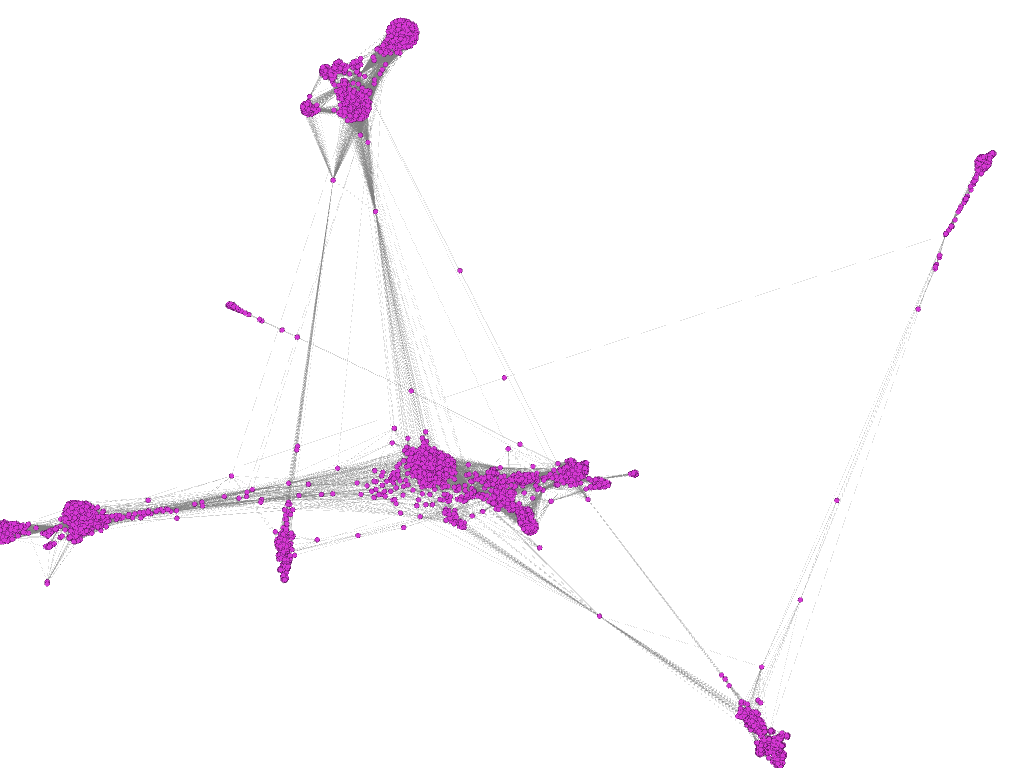
\includegraphics[width=10cm,height=10cm]{facebookGraph}}
}}}
\end{figure}
\begin{description}
\item [{5.Graph}] visualization
\end{description}
After all files are exported, inicialize Gephi. Once it starts, you
will see a welcome window, select \textbf{\textit{\textcolor{black}{``Open
graph file''}}}. Go to your directory where you have all the exported
files and select one. Once you have selected the file, a new window
will appear with all the graph information. After you select \textbf{\textit{\textcolor{black}{``Ok''}}}
your graph will be created.
\begin{description}
\item [{6.Advantages}] and Disadvantages of Graph viewers
\end{description}
The main advantage of using a graph viewer, is the easy manipulation
and visualization of graphs. This type of tools allows you to see
not only the graph, but also all the data stored in them. It also
allows you to aply filters to visualize the information you need in
each case. 

At the moment, most tools as it is the case of Gephi, do not support
hipergraphs, making it its main disadvantage. 
\begin{description}
\item [{7.Code}]~
\end{description}
If you wish to see the code, it is available in a github repository,
justo go to \textbf{\textit{\textcolor{black}{https://github.com/alejandratub/Algoritmos/
tarea4. }}}There you will find all exporting functions and files created
after the export. 
\begin{thebibliography}{10}
\bibitem{key-2}\textit{\textcolor{black}{\footnotesize{}1. GEFX Working
Group, GEFX File Format, Gephi Comunity Project, 2009.}}{\footnotesize \par}

\bibitem{key-3}\textit{\textcolor{black}{\footnotesize{}2. GraphML
team, The GrapML File Format, Graph Drawing, 2016.}}{\footnotesize \par}

\bibitem{key-4}\textit{\textcolor{black}{\footnotesize{}3. Jbmusso,
GraphSON Reader and Writer Library, Github, 2016.}}{\footnotesize \par}

\bibitem{key-5}\textit{\textcolor{black}{\footnotesize{}4. Gephi,
GDF Format, Gephi, 2017.}}{\footnotesize \par}

\bibitem{key-6}\textit{\textcolor{black}{\footnotesize{}5. Lyx, Lyx
the Document Processor, Lyx, 1995.}}{\footnotesize \par}

\bibitem{key-7}{\footnotesize{}6. Jos� Federico Medrano, Jos� Luis
Alonso Berrocal and Carlos G. Figuerola, Visualizaci�n de Grafos Web,
Universidad de Salamanca, 2011.}{\footnotesize \par}

\bibitem{key-8}{\footnotesize{}7. Doxygen, SNAP Library 4.0, User
Reference, Stanford University, 2017.}{\footnotesize \par}

\bibitem{key-9}{\footnotesize{}8. Jure Leskovec, Stanford Large Network
Dataset Collection, Stanford University, 2004.}{\footnotesize \par}

\bibitem{key-10}\textit{\textcolor{black}{\footnotesize{}9. Javier
Bezos, LaTex, Wikipedia, 2017.}}{\footnotesize \par}

\bibitem{key-13}\textit{\textcolor{black}{\footnotesize{}10. LaTex
Project, LaTeX \textendash{} A document preparation system, The LaTex
Project, 2017.}}{\footnotesize \par}

\bibitem{key-12}\textit{\textcolor{black}{\footnotesize{}11. Ulrik
Brandes and Christian Pich, GraphML Transformation, University of
Konstanz, 2010.}}{\footnotesize \par}

\bibitem{key-11}\textit{\textcolor{black}{\footnotesize{}12. yWorks
GmbH, Graph Exchange and Graph Export Formats, yWorks, 2016.}}{\footnotesize \par}
\end{thebibliography}

\end{document}
